
%(BEGIN_QUESTION)
% Copyright 2007, Tony R. Kuphaldt, released under the Creative Commons Attribution License (v 1.0)
% This means you may do almost anything with this work of mine, so long as you give me proper credit

Explain how the following annunciator circuit works:

$$\includegraphics[width=15.5cm]{i02249x01.eps}$$

Note the jumper options shown in the diagram: one set of jumper positions configures the alarm for a process switch that alarms when its contacts open, and the other positions configures the alarm for a process switch that alarms when its contacts close.  In either case, the circuit is designed to indicate an alarm status when the line going in to the lower-left NAND gate goes {\it high}.

\underbar{file i02249}
%(END_QUESTION)





%(BEGIN_ANSWER)

The first two (left-most) NAND gates form an active-low S-R latch circuit.  That is, a ``low'' state on the upper input (from the acknowledge switch) {\it sets} the S-R latch so that the upper NAND gate outputs a high signal, and a ``low'' state on the lower input (process switch returning to a non-alarm condition) ``resets'' the S-R latch so that the lower NAND gate outputs a high signal.  Thus, the purpose of the S-R latch is to remember the ``acknowledged'' status of the alarm point.  Actuating the ``Ack'' switch sets the latch and acknowledges the alarm.  Having the process switch return to a normal (non-alarm) status resets the latch and prepares the circuit for full alert (flashing light and pulsing buzzer) for the next alarm state.

%(END_ANSWER)





%(BEGIN_NOTES)

This makes a great student project, for refreshing their understanding of logic gate operation!

\vskip 20pt \vbox{\hrule \hbox{\strut \vrule{} {\bf Virtual Troubleshooting} \vrule} \hrule}

This question is a good candidate for a ``Virtual Troubleshooting'' exercise.  Presenting the diagram to students, you first imagine in your own mind a particular fault in the system.  Then, you present one or more symptoms of that fault (something noticeable by an operator or other user of the system).  Students then propose various diagnostic tests to perform on this system to identify the nature and location of the fault, as though they were technicians trying to troubleshoot the problem.  Your job is to tell them what the result(s) would be for each of the proposed diagnostic tests, documenting those results where all the students can see.

During and after the exercise, it is good to ask students follow-up questions such as:

\begin{itemize}
\item{} What does the result of the last diagnostic test tell you about the fault?
\item{} Suppose the results of the last diagnostic test were different.  What then would that result tell you about the fault?
\item{} Is the last diagnostic test the best one we could do?
\item{} What would be the ideal order of tests, to diagnose the problem in as few steps as possible?
\end{itemize}

%INDEX% Alarm, annunciator: digital circuit 

%(END_NOTES)


